\section*{Methods}
\label{sec:methods}

To probe the performance of the DNN model in various scenarios we start from a default model \cite{web:ref_notebooks}. We choose a feed-forward fully-connected neural network, with three hidden layers, one of which is a dropout layer. The model is built in Keras, on the full specifications listed in Table \ref{tab:default_model}. The performance of the model is evaluated on the binary classifier accuracy
\[ \text{Accuracy} = \frac{ \text{True Positives} + \text{True Negatives}}{\text{number of samples}}\]
and the loss function is the commonly used \texttt{binary\_crossentropy}.

\begin{table}[t]
\begin{tabular}{ccccc}
\hline\hline layer    & type    & outputs & parameters & activation\\ \hline
input    & Dense   & 2       & 6     & ReLU     \\
dense\_1 & Dense   & 20      & 60    & ReLU     \\
dense\_2 & Dense   & 20      & 420   & ReLU     \\
dropout  & Dropout & 20      & 0     & -        \\
output   & Dense   & 1       & 21    & sigmoid  \\ \hline\hline
\multicolumn{3}{c}{dropout rate}  & \multicolumn{2}{c}{0.2} \\
\multicolumn{3}{c}{optimizer}  & \multicolumn{2}{c}{adam} \\ \hline\hline
\end{tabular}
\caption{\label{tab:default_model}Layout of the default model for our DNN. This configuration corresponds to a total of 507 trainable parameters.} %In a typical scenario, the model is trained for 400 epochs with a batch-size of 100. However these values may change accordingly to the specific context.
\end{table}

This default configuration is exploited all through the next section of this report. In section \ref{sec:gridsearches} we will discuss the impact of optimizer and activation functions, as well as the layer configuration. The section \ref{sec:data_init} accounts for a brief analysis about the role of data rescaling and weight initialization methods. Ultimately, in section \ref{sec:more_patterns} we will use an optimal model, derived using the information presented in the previous sections, to test the accuracy on more complex data patterns.


\subsection{The reference training dataset}
\label{ssec:standard_dataset}

The datasets we exploit consist in several thousands of 2-dimensional points $\vec{x}$, labelled according to a pattern function $y = f(\vec{x}) \in \{0,1\}$. At first, we create reference dataset generating 4000 random points in the domain $[-50, 50]^2$, applying a pattern function that visually resembles a trimmed \emph{triangle}, as shown in Figures \ref{fig:predictions}, on the left. We choose to use $80\%$ of the dataset as the training set. For instance, the 4000 points of the reference dataset will be splitted in $3200$ samples for training, and $800$ for validation.

%\begin{figure}[h]
%  \centering
%  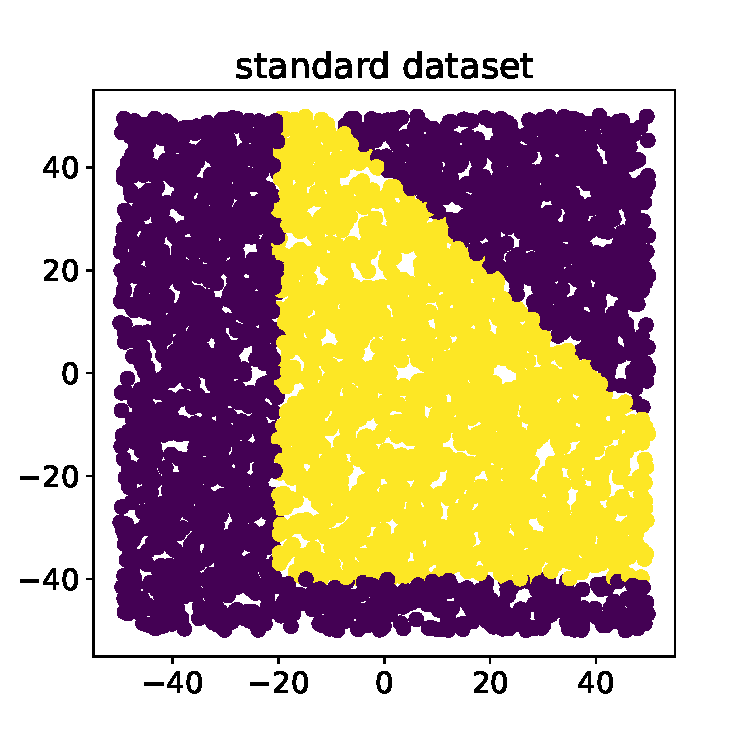
\includegraphics[width=0.7\columnwidth]{dataset_std.pdf}
%  \caption{\label{fig:dataset_std} The standard pattern function probed in this report, the %\texttt{'triangle'}. The two colors correspond to different labels of the data.}
%\end{figure}